\subsection{Kern einer Funktion}
Sei $f:{A}\longrightarrow{B}$ eine Abbildungsvorschrift.
Dann ist die Menge
\begin{align*}
   \ker(f) := \{(a,b) | f(a)=f(b)\} %Interessant: \ker ist bereits definiert!
\end{align*}
der sogenannte Kern von f.
Umgangssprachlich ausgedrückt: Alle Paare, die den selben Funktionswert besitzen.
\subsubsection{Beispiel}
\begin{align*}
  f: &\mathbb{R} \rightarrow \mathbb{R} : {x}\longmapsto{x^2} \\
  \ker(f) &= \{(a,b) | f(a)=f(b) \} \\
         &= \{ (a,b) | a^2 = b^2 \} \\
         &= \{ (a,b) | |a| =|b| \}
\end{align*}
Ein anschaulicher Erklärungsversuch: Um den Kern dieser Funktion zu bestimmen, zeichnet man eine Parallele zur X-Achse zum Graph der Funktion(vgl. Grafik).
Nun untersucht man an der Stelle a, welche Werte den den selben Funktionswert besitzen. Offensichtlich trifft die Parallele zur X-Achse den Graph wiederrum bei -a. 
Also muss die Menge $\{(0,0),(1,-1),(-1,1),(2,-2), ...\} = \{ (a,-a) | a \in \mathbb{R} \}$ Teil des Kerns sein.
Außerdem muss(wie unter \ref{kern_eigenschaften} erläutert wird) auch die Menge $\{(a,a) | a \in \mathbb{R} \}$ im Kern enthalten sein, was insgesamt zu obigem Ergebnis führt. 
\begin{center}
 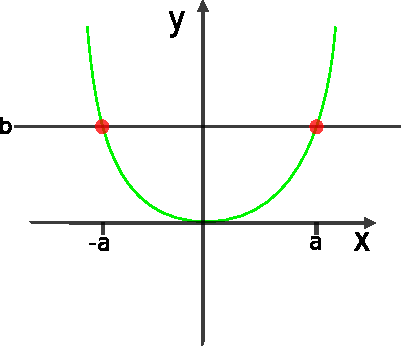
\includegraphics[keepaspectratio=true]{../bilder/parabel_kernsvg.pdf}
 % parabel_kernsvg.pdf: 194x166 pixel, 72dpi, 6.84x5.86 cm, bb=0 0 194 166
\end{center}

\subsubsection{Rechnerische Behandlung}
Je nach Abbildung kann man den Kern auch rechnerisch bestimmen. Hierfür soll das Beispiel noch einmal etwas ausführlicher erläutert werden.
Der Ausgangspunkt ist, dass zwei (nicht notwendigerweise verschiedene) Werte $x_1, x_2$ auf das selbe Element abgebildet werden sollen:
$$  f(x_1) = f(x_2) $$
$$ {x_1}^2 = {x_2}^2$$
Wurzelziehen führt zu den Lösungen
$ x_1 = x_2 $ sowie $ x_1 = - x_2 $
Dieses Beispiel ist rechnerisch recht trivial, entscheident ist, dass man den Ansatz verstanden hat: 
man muss für (möglicherweise unterschiedliche) Werte beim Einsetzen in die Funktion das selbe Ergebnis erhalten.
\footnote{Wenn gewünscht, kann man hier auch ein etwas komplexeres Beispiel (so wie das in der Übung z.B.) einfügen. Sagt einfach irgendwie Bescheid, wenn Bedarf besteht.}


\subsubsection{Eigenschaften des Kerns}\label{kern_eigenschaften} 
Wegen $ f(a) = f(a) $ muss $\ker(f)$ immer $\{(a,a) | a \in {A} \}$ enthalten.
Anders formuliert: da man bei einer Funktion für ein und den selben Eingabewert immer das selbe herrausbekommt, müssen diese im Kern enthalten sein.

% Brauch mein Emacs um das Masterfile zu finden
%%% Local Variables:
%%% mode: latex
%%% TeX-master: "../script"
%%% End:
